
%(BEGIN_QUESTION)
% Copyright 2009, Tony R. Kuphaldt, released under the Creative Commons Attribution License (v 1.0)
% This means you may do almost anything with this work of mine, so long as you give me proper credit

In this process, maple syrup is heated as it passes through a steam heat exchanger, then enters an evaporator where the water boils off.  The purpose of this is to raise the sugar concentration of the syrup, making it suitable for use as a food topping.  A level control system (LT, LIC, and LV) maintains constant syrup level inside the evaporator, while an analytical control system (AT, AIR, AC, and AV) monitors the sugar concentration of the syrup and adjusts steam flow to the heat exchanger accordingly.

$$\includegraphics[width=15.5cm]{i02935x01.eps}$$

Suppose a process operator accidently leaves the manual block valve {\it locked} and {\it tagged} shut following an overhaul of the process, so that no steam can enter the heat exchanger.  Describe how both control systems will respond over time to this process condition.

\vskip 20pt \vbox{\hrule \hbox{\strut \vrule{} {\bf Suggestions for Socratic discussion} \vrule} \hrule}

\begin{itemize}
\item{} Explain the function of a {\it heat exchanger}, describing its construction as well.
\item{} Why do you think it is important to monitor and control the level of syrup inside the evaporator?
\item{} How realistic do you think it is that a person might accidently leave their lock and tag on a closed valve following a long period of down-time?
\end{itemize}

\underbar{file i02935}
%(END_QUESTION)





%(BEGIN_ANSWER)

%(END_ANSWER)





%(BEGIN_NOTES)

The analytical controller will drive the steam valve wide open (to no effect, though).  The level controller will operate normally, maintaining syrup level inside the evaporator at setpoint.

\vskip 10pt

The level control valve may need to open up further than usual, since a greater liquid flow will now exit the evaporator (no water being driven off the syrup).  However, the effluent will be a lot less viscous than before since the water content is greater, and this may very well affect the valve opening (not having to be open as wide as if the greater flow had the same viscosity as the original flow).

\vskip 20pt \vbox{\hrule \hbox{\strut \vrule{} {\bf Virtual Troubleshooting} \vrule} \hrule}

This question is a good candidate for a ``Virtual Troubleshooting'' exercise.  Presenting the diagram to students, you first imagine in your own mind a particular fault in the system.  Then, you present one or more symptoms of that fault (something noticeable by an operator or other user of the system).  Students then propose various diagnostic tests to perform on this system to identify the nature and location of the fault, as though they were technicians trying to troubleshoot the problem.  Your job is to tell them what the result(s) would be for each of the proposed diagnostic tests, documenting those results where all the students can see.

During and after the exercise, it is good to ask students follow-up questions such as:

\begin{itemize}
\item{} What does the result of the last diagnostic test tell you about the fault?
\item{} Suppose the results of the last diagnostic test were different.  What then would that result tell you about the fault?
\item{} Is the last diagnostic test the best one we could do?
\item{} What would be the ideal order of tests, to diagnose the problem in as few steps as possible?
\end{itemize}

%INDEX% Basics, control loop troubleshooting: determining effect of process valve problem
%INDEX% Process: maple syrup concentration (single-effect evaporator)

%(END_NOTES)


